%\documentclass[a4paper,10pt]{article}

%\documentclass[russian,utf8,emptystyle, pointsection, 14pt]{eskdtext}
\documentclass[russian,utf8, pointsubsection]{eskdtext}
%\usepackage{eskdplain}
\usepackage[utf8]{inputenc}
\usepackage[russian]{babel}

\usepackage[T2A]{fontenc}
\usepackage{hyperref}
\hypersetup{colorlinks=true, linkcolor=blue,
citecolor=blue, filecolor=blue, urlcolor=blue, pdftitle=}

\usepackage{graphics}
\usepackage{longtable}
%\usepackage{lscape}
\usepackage[pdftex]{lscape}

%\usepackage{pdflscape}

%\bibliographystyle{utf8gost705u}

\usepackage{eskdchngsheet}
%\usepackage{python}
\usepackage{multirow}
\usepackage{amsmath}
\usepackage{cite}
% \usepackage{tocloft}
\usepackage{amsfonts}
\usepackage{amssymb}
\usepackage{pdfpages}
\usepackage{booktabs} % For \toprule, \midrule and \bottomrule
\usepackage{siunitx} % Formats the units and values
\usepackage{pgfplotstable} % Generates table from .csv
\usepackage{cmap}
\usepackage{color} \definecolor{darkgreen}{rgb}{0,.5,0}
%\usepackage[unicode,colorlinks,filecolor=blue,citecolor=darkgreen]{hyperref}
\usepackage{lscape}
\usepackage{eskdfreesize}
%\usepackage[T2A]{fontenc}
%\usepackage{pscyr}
\sisetup{
  round-mode          = places, % Rounds numbers
  round-precision     = 2, % to 2 places
}

\renewcommand{\ESKDagreedName}{%
  \cyr\CYRS\CYRO\CYRG\CYRL\CYRA\CYRS\CYRO\CYRV\CYRA\CYRN\CYRO} % "СОГЛАСОВАНО" заглавными
\renewcommand{\ESKDapprovingName}{%
  \cyr\CYRU\CYRT\CYRV\CYRE\CYRR\CYRZH\CYRD\CYRA\CYRYU} % "УТВЕРЖДАЮ" заглавными
\renewcommand{\ESKDapprovedName}{%
   \cyr\CYRU\CYRT\CYRV\CYRE\CYRR\CYRZH\CYRD\CYRE\CYRN} % "УТВЕРЖДЕН" заглавными
\renewcommand{\ESKDapprovingSheetName}{%
  \cyr\CYRL\cyri\cyrs\cyrt\ %
  \cyru\cyrt\cyrv\cyre\cyrr\cyrzh\cyrd\cyre\cyrn\cyri\cyrya}

%\ESKDcompany{ПАО <<ПРОТОН-ПМ>>}
%\ESKDgroup{ПАО <<ПРОТОН-ПМ>>}
\ESKDcompany{ООО НТЦ <<ТУРБОПНЕВМАТИК>>}
\ESKDgroup{ООО НТЦ <<ТУРБОПНЕВМАТИК>>}
%\ESKDtitleApprovedBy{Главный инженер}{Т. Н. Компанец}
\ESKDtitleApprovedBy{Технический директор}{А. А. Снитко}

\ESKDauthor{Целищев}
\ESKDchecker{}
\ESKDnormContr{}
\ESKDapprovedBy{}

%\ESKDtitleAgreedBy{Начальник 209 ВП МО РФ}{А. И. Бодак}
%\ESKDtitleDesignedBy {Главный технолог}{А. А. Целищев}
\ESKDtitleDesignedBy {Начальник теплотехнического отдела}{А. А. Целищев}
%\ESKDtitleAgreedBy {Нач. отдела надежности}{Д. А. Новиков}
%\ESKDtitleDesignedBy {Ведущий специалист-конструктор-расчетчик}{А. А. Целищев}
%\ESKDtitleDesignedBy {Специалист-конструктор-расчетчик}{В. В. Пшеничный}

\renewcommand{\ESKDtheTitleFieldX}{} % Убрана дата с титульного листа

\renewcommand{\ESKDsectionStyle}{\normalfont\Large\bfseries\MakeUppercase}
\renewcommand{\ESKDsubsectionStyle}{\normalfont\large\bfseries}
\renewcommand{\ESKDsubsubsectionStyle}{\normalfont\normalsize\bfseries}

%\ESKDsectStyle{\section}{\textsc}
%
\newcommand{\No}{\textnumero}
\newcommand{\no}{\textnumero}
\newcommand{\cels}{~$^0C$}
\newcommand{\obmin}{~об/мин}
\newcommand{\mpa}{~МПа}
\newcommand{\kgscm}{~кгс/см$^2$}
\newcommand{\kgsm}{~кгс$\cdot$м}
\newcommand{\kgsmm}{~кгс/мм$^2$}
\newcommand{\kJ}{~кДж}
\newcommand{\J}{~Дж}
\newcommand{\pa}{~Па}
\newcommand{\mm}{~мм}
\newcommand{\kpa}{~кПа}
\newcommand{\ms}{~м/с}
\newcommand{\watt}{~Вт}
\newcommand{\kwatt}{~кВт}
\newcommand{\megawatt}{~MВт}
\newcommand{\qm}{~м$^2$}
\newcommand{\qmm}{~мм$^2$}
\newcommand{\grad}{~$^0C$}
\newcommand{\minut}{~'}
\newcommand{\secund}{~'}

\bibliographystyle{gost2003s}
\setcounter{tocdepth}{2}
%
%\renewcommand{\l@subsection}{\@tocline{2}{0.8cm}{0.8cm}}
\usepackage{soul}
\makeatletter \renewcommand{\@dotsep}{10000} \makeatother % Исключены точки в оглавлении
% \renewcommand{\l@section}{\@dottedtocline{1}{1.5em}{2.3em}}
% \renewcommand{\l@subsection}{\@dottedtocline{2}{1.5em}{2.3em}}
% \renewcommand{\l@subsubsection}{\@dottedtocline{2}{1.5em}{2.3em}}

%\renewcommand{\part}[1]{#1 \refstepcounter{}

%\renewcommand{\thesection}{\thepart.\arabic{section}}

\newcommand{\thepointsection}{\thesection.\arabic{subsection}}
\newcommand{\pointsection}{%
  \par\refstepcounter{subsection}\thepointsection\quad}

\newcommand{\thepointsubsection}{\thesubsection.\arabic{subsubsection}}
\newcommand{\pointsubsection}{%
  \par\refstepcounter{subsubsection}\thepointsubsection\quad}

\newcounter{subsubsubsection}[subsubsection]

\newcommand{\thepointsubsubsection}{\thesubsubsection.\arabic{subsubsubsection}}
\newcommand{\pointsubsubsection}{%
  \par\refstepcounter{subsubsubsection}\thepointsubsubsection\quad}

%создание и автоматическая нумерация списков
\RequirePackage{enumitem}
\renewcommand{\alph}[1]{\asbuk{#1}} % костыль для кирилической нумерации вместо латинской

\setlist{nolistsep} % убираем дополнительные вертикальные отступы вокруг списков
\setenumerate[1]{label=\alph*), fullwidth, itemindent=\parindent,  listparindent=\parindent} 
\setenumerate[2]{label=\arabic*), fullwidth, itemindent=\parindent, listparindent=\parindent, leftmargin=\parindent}

\setitemize{fullwidth, itemindent=\parindent, listparindent=\parindent}

% Настраиваем шрифт разделов в оглавлении
\makeatletter
\renewcommand{\l@section}{\bfseries \@dottedtocline{1}{0em}{1.5em}}
\renewcommand{\l@subsection}{\normalfont \@dottedtocline{2}{0em}{2.5em}}
\makeatother

\ESKDcolumnIX{\small{ООО НТЦ <<ТУРБОПНЕВМАТИК>>}}
\title{ТРЕБОВАНИЯ К ЧИСТОТЕ ИЗДЕЛИЙ}
\ESKDdocName{Инструкция}
\ESKDsignature{ГРФМ.0000.000.000И001}
\ESKDtitleApprovingSheet{ГРФМ.0000.000.000И001ЛУ}
\ESKDchecker{Пеков}
\makeindex

\usepackage{Sweave}
\begin{document}
\Sconcordance{concordance:main.tex:main.Rnw:%
1 31 1 1 0 80 1}

\maketitle

%\ESKDapprovingDoc{fff}

%\maketitle
\tableofcontents

\newpage
\section{Введение}
\section{Цели}
\pointsection Выбор и определение параметров расчетной модели
\pointsection \label{sec:limits} Определение сопротивления движению груза даунриггера при подводном движении на скоростях от 0.5 до 2~м/с с заглублением от 0.5 до 50 метров с нормальной температурой среды, с учетом удерживающего троса диаметром 1~мм.;
\pointsection Определение устойчивости движения груза дауриггера во всем диаппазоне приведенном в п. \ref{sec:limits}.

\section{Выводы}
\section{Рекомендации}
\section{Заключение}
\section{Содержание отчета}
\subsection{Исходные данные и описание работы}

Груз даунриггера применяется для заглубления и стабидизации глубины движения приманки при рыбной ловле на глубинах от 2 до 20 метров при скоростях движения судна  от 0.5 до 2~м/с. Общий вид груза даунрингера приведен на рисунке~\ref{ris:allView}.

Поскольку ловля с помощью даунриггера производится в летнее время, а характеристики воды в открытых водоемах изменяются незначительно, то расчеты выполним при температуре воды 15\cels. 

\begin{figure}[h]
\center{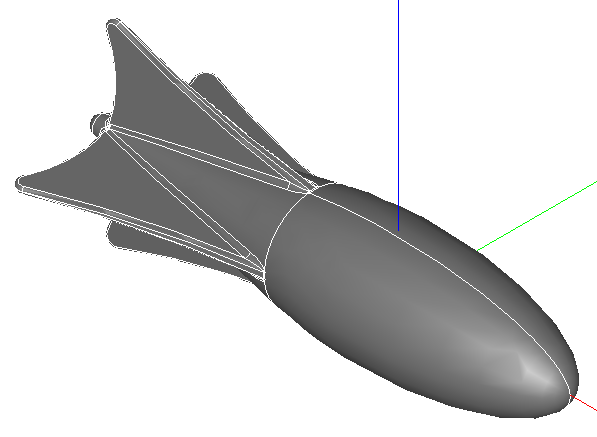
\includegraphics[width=1\linewidth]{pic/fullViewEdited.png}}
\caption{Общий вид модели груза даунриггера}
\label{ris:allView}
\end{figure}



\subsection{Выбор и валидация расчетной модели}

Поскольку точные данные по лобовому сопротивлению груза даунриггера отсутсвуют, то для разработки расчетной сетки используем доступные экспериментальные данные по лобовому сопротивлению:
\begin{itemize}
\item обтекании цилиндра при направлении вектора набегающего потока направленном под прямым углом к оси цилиндра~\cite{cylInFlow};
\end{itemize}

При движении груза необходимо учитывать удельное (по глубине погружения) сопротивлеие троса подвеса груза. В этом случае модель сопротивления, изложенная в \cite{cylInFlow}, может также использоваться для валидации применяемой модели и коэффициентов. 


\subsection{Определение основных характеристик}

\subsubsection{Определение основных характеристик среды и режима движения жидкости}
Для воды в нормальных условиях характеристики жидкости:
\begin{enumerate}
\item плотность, кг/м$^2$: 1000
\item динамическая вязкость, $\text{Па}\cdot\text{с}$: $1006\cdot10^{-6}$; \cite{waterProps}
\item кинематическая вязкость, $\text{м}^2/\text{с}$: $1.006\cdot10^{-6}$ \cite{waterProps}
\end{enumerate}

\subsubsection{Определение основных характеристик движения жидкости}
В качестве характерного размера даунриггера примем максимальльный диаметр <<тела>>, равный 0.05~м. Для этого характерного размера число Рейнолдса равно:

\begin{equation}
Re = \frac{u\cdot{L}}{\nu} 
\end{equation}

По расчету:
\begin{equation}
Re = \frac{(0,5\dots2)\cdot{0,05}}{1.006\cdot10^{-6}}=24850,89\dots99403,58
\end{equation}

Исходя из числа Рейнолдса видно, что движение жидкости при обтекании груза даунриггера турбулентное.

Характерный размер подвесного троса --- диаметр, равный $0.0005\dots0.001$~м. Для этого характерного размера число Рейнолдса равно:

\begin{equation}
Re = \frac{(0,5\dots2)\cdot{(0,0005\dots0.001)}}{1.006\cdot10^{-6}}=248,509\dots1988,07
\end{equation}

Исходя из числа Рейнолдса видно, что движение жидкости при обтекании троса подвеса переходное, от ламинарного к турбулентному.



\bibliographystyle{unsrt}
\bibliography{my_all}
\end{document}
